\documentclass[pdf,aspectratio=169]{beamer}
\usepackage[]{hyperref,graphicx,siunitx,booktabs,lmodern}
\usepackage{physics}
\usepackage{em-commands}
\mode<presentation>{\usetheme{EM}}

%Question Numbering
\newcounter{questionnumber}
\newcommand{\qnum}{%
	\stepcounter{questionnumber}%
	Q\arabic{questionnumber}
}
\resetcounteronoverlays{questionnumber}

\graphicspath{ {../Images/} }

\sisetup{per-mode=symbol}

\tikzstyle{plate}=[draw, very thick, minimum width=4cm, minimum height=1cm, fill=gray!40, anchor=south]

%preamble
\title{Happy Chaper Day!}
\date{October 17, 2018}
\author{Jed Rembold}

\begin{document}
\renewcommand{\theenumi}{\Alph{enumi}}

\begin{frame}{Announcements}
	\begin{itemize}
		\item Happy Chaper Day!!
		\item Still working on the tests, sorry
		\item Homework 7 is due on Monday!
		\item Physics Club on Thursday at 4:30pm
			\begin{itemize}
				\item Nobody showed last week, so there goes my faith in you being able to solve the world's problems\ldots
				\item This week it gets easier. 
					Solving mazes using a computer. 
					Brought to you by me. 
				\item \url{http://jrembold.github.io/code_challenge}
			\end{itemize}
			
		\item No class on Friday!
	\end{itemize}
\end{frame}

\begin{frame}{\qnum}
	On Monday we saw that, for the case of the electret, despite there being no free charges present, $\ef\neq 0$ and thus $\va{D}\neq 0$.
	Since $\div \va{D} = \rho_{free}$, this implies that $\curl \va{D} \neq 0$. Where is there a non-zero value of the curl of $\va{D}$ in this problem?
	\begin{enumerate}
		\item In the center of the cylinder
		\item At the top surface
		\item At the bottom surface
		\item \alert<2>{Just outside the cylinder}
	\end{enumerate}
\end{frame}

\begin{frame}{\qnum}
	A very large (basically infinite) capacitor has charge $Q$.
	A neutral dielectric is inserted into the gap (and it will of course then polarize). 
	We want to find $\va{D}$ everywhere.

	\begin{columns}
		\column{0.5\textwidth}
		Which equation would you head to first?
		\begin{enumerate}
			\item $\ed = \epsilon_0\ef + \pol$
			\item \alert<2>{$\oint \ed\vdot d\vA = Q_{free}$}
			\item $\oint \ef\vdot d\vA = \tfrac{Q}{\epsilon_0}$
			\item More than one of these would work
		\end{enumerate}
		
		\column{0.5\textwidth}
		\begin{center}
			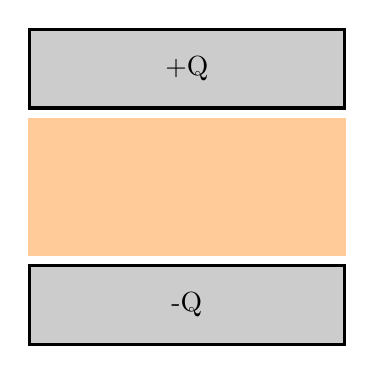
\begin{tikzpicture}
				\node[plate] (np) at (0,0) {-Q};
				\node[plate] (pp) at (0,3) {+Q};
				\fill[orange!40] ([yshift=1mm]np.north west) rectangle ([yshift=-1mm]pp.south east);
			\end{tikzpicture}
		\end{center}
	\end{columns}
\end{frame}

\begin{frame}{\qnum}
	\begin{columns}
		\column{0.5\textwidth}
		A large capacitor has charge $Q$.
		A neutral linear dielectric is inserted into the gap. 
		We want to find $\ed$ in the dielectric.
		
		For the Gaussian cube shown, what is $Q_{free, enclosed}$?
		\begin{enumerate}
			\item \alert<2>{$\sigma \ell^2$}
			\item $-\sigma_b \ell^2$
			\item $(\sigma-\sigma_b)\ell^2$
			\item $(\sigma+\sigma_b)\ell^2$
		\end{enumerate}
		\column{0.4\textwidth}
		\begin{center}
			\begin{tikzpicture}
				\node[plate] (np) at (0,0) {};
				\node[plate] (pp) at (0,3) {};
				\node[above,math] at (pp.200) {+\sigma};
				\node[below,math] at (np.160) {-\sigma};
				\fill[orange!40] ([yshift=1mm]np.north west) rectangle ([yshift=-1mm]pp.south east);
				\node[above,math] at (np.160) {+\sigma_b};
				\node[below,math] at (pp.200) {-\sigma_b};
				\draw[very thick, dashed] ([xshift=-.7cm,yshift=-.7cm]pp.south) rectangle +(1.4,1.4);
				\node at ([yshift=-1cm]pp.south) {$\ell$};
			\end{tikzpicture}
		\end{center}
		
	\end{columns}
\end{frame}

\begin{frame}{\qnum}
	\begin{columns}
		\column{0.5\textwidth}
		A large capacitor has charge $Q$.
		A neutral linear dielectric is inserted into the gap. 
		We want to find $\ed$ in the dielectric.
		
		Is $\ed$ zero inside the metal?
		\begin{enumerate}
			\item \alert<2>{It must be zero in there.}
			\item It depends.
			\item It is definitely \emph{not} zero in there.
		\end{enumerate}
		\column{0.4\textwidth}
		\begin{center}
			\begin{tikzpicture}
				\node[plate] (np) at (0,0) {};
				\node[plate] (pp) at (0,3) {};
				\node[above,math] at (pp.200) {+\sigma};
				\node[below,math] at (np.160) {-\sigma};
				\fill[orange!40] ([yshift=1mm]np.north west) rectangle ([yshift=-1mm]pp.south east);
				\node[above,math] at (np.160) {+\sigma_b};
				\node[below,math] at (pp.200) {-\sigma_b};
				\draw[very thick, dashed] ([xshift=-.7cm,yshift=-.7cm]pp.south) rectangle +(1.4,1.4);
				\node at ([yshift=-1cm]pp.south) {$\ell$};
			\end{tikzpicture}
		\end{center}
		
	\end{columns}
\end{frame}

\begin{frame}{\qnum}
	\begin{columns}
		\column{0.5\textwidth}
		A large capacitor has charge $Q$.
		A neutral linear dielectric with dielectric constant $\epsilon_r$ is inserted into the gap. 
		
		What is the electric field inside the dielectric?
		\begin{enumerate}
			\item \alert<2>{$\displaystyle E = \frac{\sigma}{\epsilon_0\epsilon_r}$}
			\item $\displaystyle E = \frac{\sigma}{2\epsilon_0\epsilon_r}$
			\item $\displaystyle E = \frac{\sigma\epsilon_r}{2\epsilon_0}$
			\item $\displaystyle E = \frac{2\sigma\epsilon_r}{\epsilon_0}$
		\end{enumerate}
		\column{0.4\textwidth}
		\begin{center}
			\begin{tikzpicture}
				\node[plate] (np) at (0,0) {};
				\node[plate] (pp) at (0,3) {};
				\node[above,math] at (pp.200) {+\sigma};
				\node[below,math] at (np.160) {-\sigma};
				\fill[orange!40] ([yshift=1mm]np.north west) rectangle ([yshift=-1mm]pp.south east);
				\node[above,math] at (np.160) {+\sigma_b};
				\node[below,math] at (pp.200) {-\sigma_b};
				\draw[very thick, dashed] ([xshift=-.7cm,yshift=-.7cm]pp.south) rectangle +(1.4,1.4);
				\node at ([yshift=-1cm]pp.south) {$\ell$};
			\end{tikzpicture}
		\end{center}
	\end{columns}
\end{frame}

%\begin{frame}{\qnum}
	%A point charge $+q$ is placed at the center of a neutral, linear homogeneous dielectric teflon spherical shell. Can $\ed$ be computed from its divergence?
	%\[\oint \ed\vdot d\vA = Q_{free}\]
	%\vspace*{-1.5cm}
	%\begin{columns}
		%\column{0.5\textwidth}
		%\begin{center}
			%\begin{tikzpicture}
				%\node[pcharge] at (0,0) {$+q$};
				%\draw[fill=orange!40, even odd rule] (0,0) circle (2) circle (3);
			%\end{tikzpicture}
		%\end{center}
		%\column{0.5\textwidth}
		%\begin{enumerate}
			%\item Yes
			%\item No
			%\item Depends on information not given
		%\end{enumerate}
	%\end{columns}
%\end{frame}

%\begin{frame}{\qnum}
	%A point charge $+q$ is placed at the center of a neutral, linear, homogeneous, dielectric hemispherical shell. Can $\ed$ be computed from its divergence?
	%\begin{columns}
		%\column{0.5\textwidth}
		%\begin{center}
			%\begin{tikzpicture}
				%\node[pcharge] at (0,0) {$+q$};
				%\draw[fill=orange!40] (-2,0) arc (180:0:2) -- ++(1,0) arc(0:180:3) -- cycle;
			%\end{tikzpicture}
		%\end{center}
		%\column{0.5\textwidth}
		%\begin{enumerate}
			%\item Yes
			%\item No
			%\item Depends on information not given
		%\end{enumerate}
	%\end{columns}
%\end{frame}










\end{document}
